\documentclass{kththesis}

\usepackage{csquotes} % Recommended by biblatex
\usepackage[style=numeric,sorting=none,backend=biber, urldate=long, dateabbrev=false]{biblatex}
\usepackage{svg}        % svg files
\usepackage{hyperref}   % clickable ToB and references
\hypersetup{
    colorlinks,
    hidelinks,
    allcolors=black
}
\usepackage[section]{placeins}

%  --- Table for scenarios ---
% https://tex.stackexchange.com/questions/431473/how-to-make-a-comparison-table-with-check
\usepackage{pifont}
\usepackage{xcolor}
\newcommand{\cmark}{\textcolor{green!80!black}{\ding{51}}}
\newcommand{\xmark}{\textcolor{red}{\ding{55}}}
%  --------------------------

\makeatletter
\AtBeginDocument{%
  \expandafter\renewcommand\expandafter\subsection\expandafter{%
    \expandafter\@fb@secFB\subsection
  }%
}
\makeatother

\addbibresource{references.bib} % The file containing our references, in BibTeX format

\title{Mätning av latens för live videosamtal över omodifierad och modifierad Tor}
\author{
  \textbf{Magnus Åkerfeldt}\\
  \textbf{Carl Engelhardt}
}
\email{akerfel@kth.se, carlenge@kth.se}
\supervisor{Daniel Bosk}
\examiner{Pawel Herman}
\programme{Bachelor in Computer Science}
\school{School of Electrical Engineering and Computer Science}
\date{\today}

% Uncomment the next line to include cover generated at https://intra.kth.se/kth-cover?l=en
\kthcover{resources/kth-cover.pdf}
\begin{document}
% Frontmatter includes the titlepage, abstracts and table-of-contents
\frontmatter
\titlepage
\begin{abstract}
    Tor is an anonymity network which consists of \emph{relays} (or \emph{nodes}) dispersed over the world. By interlaying a connection with the relays it becomes more difficult to conclude who the sender and receiver is, however the latency is also increased. A user can choose to only connect via relays in a certain country, which would affect latency and anonymity.
    
    In this thesis we routed a live video calling application through Tor, and measured how much the usage of Tor increased the latency. We also explored different approaches to lower that latency by using modified versions of Tor, where the relays were strictly limited to either Sweden or Germany. Lastly we calculated the effect on anonymity the modified versions of Tor had, using several anonymity metrics.
    
    We concluded that the usage of vanilla Tor increased the median latency by 517 ms, compared to when Tor was not used. Limiting the relays to Sweden increased the median latency by 300 ms for Tor users in Sweden, i.e. the increase was reduced by 42 \%. Limiting relays to Germany had similar latency results. However, the modifications decreased the anonymity of the user when German relays were used, and even more so when Swedish relays were used, due to Sweden's smaller number of Tor users and relays. Finally, we recognized that there exist more complex methods to modify Tor which would yield better results.
\end{abstract}

\begin{otherlanguage}{swedish}
  \begin{abstract}
    Tor är ett anonymitetsnätverk som består av noder spridda över hela världen. Genom att skapa en anslutning mellan noderna blir det svårare att dra slutsatser om vem avsändaren och mottagaren är, men det leder också till att latensen ökar. En användare kan välja att bara ansluta via noder inom ett visst land, vilket påverkar latens och anonymitet.
    
    I denna avhandling kopplade vi en live videosamtalsapplikation till Tor, och mätte hur mycket användningen av Tor ökade latensen. Vi utforskade också olika tillvägagångssätt för att sänka den latensen genom att använda modifierade versioner av Tor, där noderna var strikt begränsade till antingen Sverige eller Tyskland. Slutligen beräknade vi påverkan på anonymiteten som de modifierade versionerna av Tor hade, med flera anonymitetsmått.
    
    Vi drog slutsatsen att vanilla Tor ökade medianlatensen med 517 ms, jämfört med när Tor inte användes. Att begränsa noderna till Sverige ökade medianslatensen med 300 ms för Tor-användare i Sverige, ökningen minskade alltså med 42 \%. Begränsning av noder till Tyskland hade liknande latensresultat. Modifieringarna minskade dock användarens anonymitet när tyska noder användes, och ytterligare när svenska noder användes, på grund av Sveriges mindre antal Tor-användare och noder. Slutligen insåg vi att det finns mer komplexa metoder för att modifiera Tor som skulle ge bättre resultat.
  \end{abstract}
\end{otherlanguage}

\tableofcontents

% Mainmatter is where the actual contents of the thesis goes
\mainmatter

\chapter{Introduction}
Tor is a low-latency (as opposed to high-latency) anonymity network consisting of volunteer relays dispersed over the world. A \emph{relay} (also commonly \emph{router} or \emph{node}) is a computer running Tor software which allows the computer to receive and send along requests and responses from client and server respectively. Low-latency refers to the network's ability to handle requests in near real-time, whereas high-latency networks may take more than several hours to complete a request \parencite{UnderstandingTor}. 

The low-latency aspect of Tor enables clients to use interactive applications via the network. Interactive applications can be defined as applications where a lower latency for a client's request to be completed is preferable, e.g. web browsing or instant messaging.

However, due to Tor's network structure some latency is lost in favor of anonymity. Every request made on the Tor network by default travels through three relays before being sent to the receiver, leading to a delay compared to sending the request to the receiver directly. In addition, the three relays may be placed anywhere in the world, in some cases resulting in the travel path being several times that of a direct path \parencite{TorRelaysByCountry}. Thus, while Tor is a low-latency network, it is by nature slow when seen from the perspective of a non-anonymous network, although previous studies have tried to circumvent this \parencite{CLAPS}. 

This study aims to test the Tor network's ability to handle interactive applications using latency as a measure. Specifically live video calls, where small delays are often noticeable, will be tested. A method to affect the network's latency for the client at the cost of anonymity will also be examined.

Tor is mostly used for browsing the web, and seemingly no previous studies have investigated how well it can manage live video communication. Thus we will be exploring a novel use case for Tor. This could make Tor more accessible, and potentially lead to further development of Tor. This in turn could give people a new way of privately communicating via video.

\section{Research Questions}
The research aims to answer two questions:
\begin{itemize}
    \item If a live video calling service is routed via the Tor network, what will the latency be relative to a live video calling service not routed via the Tor network?
    \item If the routed Tor relays are limited by the region of the client, how will the latency in the previous question be affected, and how will it affect anonymity?
\end{itemize}

\section{Limitations}
The limitations of this study are discussed in detail in section \ref{section:limitations}. In summary, more practical use cases could be tested; we have not performed an in-depth analysis of what the data will mean for the user experience; only some relay regions have been evaluated; we are measuring \emph{relative} latency (not \emph{absolute} latency); and we have used simplified anonymity calculations that rely on some assumptions.

\section{GitHub}
The LaTeX source code and raw data \parencite{thesisGithub}, as well as the source code for the video latency measuring program \parencite{latencyAnalyzer}, have been uploaded to GitHub.

\chapter{Background}
In this chapter the following topics will be presented:

\begin{itemize}
    \item How Tor works.
    \item Tor's path selection algorithm.
    \item Tor's transport protocol (TCP), and how it is relevant for this study.
    \item Autonomous systems, and some of Tor's anonymity vulnerabilities.
    \item Tor compared to Signal, in terms of latency and privacy.
    \item Related work that has explored methods for measuring video latency, and how the performance and anonymity for Tor could be improved by changing Tor's path selection algorithm.
\end{itemize}

\section{Tor}
Tor (lit. \emph{The onion router}) is, as mentioned, a low-latency anonymous network and consists of relays run by volunteers. When a client establishes a connection to a server through Tor, a \emph{circuit} (or \emph{path}) is created. A circuit by default consists of three relays called \emph{entry guard}, \emph{middle relay}, and \emph{exit relay}, and makes the connection between client and server. A request from the client is first sent to the entry guard, which forwards the request to the middle relay, which forwards the request to the exit relay, which sends the request to the server. The response from the server is sent back over the same circuit, but in reverse order starting with the exit relay \parencite{UnderstandingTor}. See figure \ref{fig:torCircuit}.

\begin{figure}[!htb]
    \centering
    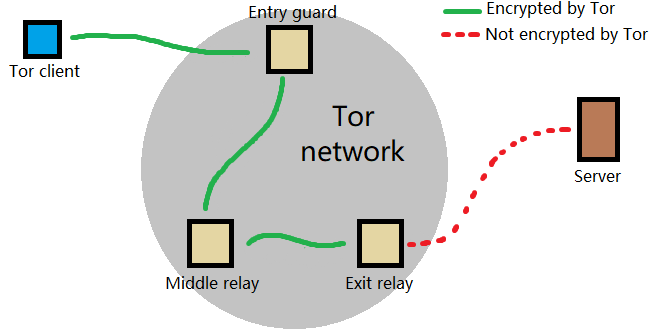
\includegraphics[width=350pt]{resources/paint_tor_circuit.png}
    \caption{An illustration of how a Tor client connects to a server through three relays in the Tor network.}
    \label{fig:torCircuit}
\end{figure}

The client request is encrypted in layers. A symmetric key is shared with each of the relays in the circuit, i.e. the client has three keys, and the relays have one each. When the client initially sends its request it is encrypted with all three keys. Each relay successively decrypts the request with their respective key, giving the exit relay the unencrypted request (note that the request may still be encrypted with for example HTTPS). The exit relay is then able to forward the request to the server. The response from the server is again managed in reverse order: starting with the exit relay, each relay encrypts the response with their symmetric key. The client then decrypts the response with its three symmetric keys \parencite{TorOnionRouter}\parencite{UnderstandingTor}.

Tor's encryption layer increases anonymity. If an adversary compromises the entry guard of a certain circuit (by either owning the entry guard or attacking it by some means), they know that the client is running Tor; if they compromise the middle relay the adversary knows nothing of the client; and if the adversary compromises the exit relay they know that \emph{someone} on Tor is visiting a certain server (assuming a HTTPS connection). However if both the entry guard relay \emph{and} the exit relay is compromised the adversary can use e.g. a \emph{Traffic Correlation Attack} \parencite{CLAPS} in order to find out which server a certain client accessed, in which case the client's anonymity is breached \parencite{TorOnionRouter}.

\section{Tor's path selection algorithm}
Tor's path selection algorithm \parencite{TorPathSpecification} selects the relays to be used for a circuit. The algorithm follows certain rules and constraints in an effort to increase anonymity and performance. For example, the algorithm avoids scenarios where an actor controls more than one relay in the same circuit; the same relay is never chosen twice for the same path; or if they are in the same /16 subnet. Tor's current path selection algorithm does not have any regional constraints.

\section{TCP and UDP}
On the transport layer, Tor only uses TCP (Transmission Control Protocol) streams \parencite{officialTorOverview} and does not support UDP (User Datagram Protocol) streams. This could be seen as a problem in the context of this project, since UDP usually is preferred over TCP for applications where low latency is of importance; for example, Zoom uses a combination of UDP and TCP \parencite{ZoomTCPandUDP}. Most other live video calling applications also rely more on UDP than TCP. This is for a multitude of reasons, one being that UDP allows for packets to be lost when sending data. For TCP, the receiver has to wait for lost packets to be re-sent and received again. Therefore, using TCP will result in higher latency.

Although Tor uses TCP, there has been a study which implemented unordered delivery for TCP on Tor \parencite{unorderedTCPdelivery}, meaning that the packets can arrive out of order as opposed to having to arrive in order. The study concluded that unordered delivery for TCP noticeably decreased the latency while not affecting anonymity.

\section{Autonomous Systems}
An \emph{Autonomous System} (or \emph{AS}) can be described as a collection of IP networks which are administered by a single entity, and have a clearly defined policy for routing \parencite{hawkinson1996guidelines}. AS:es can host Tor relays, and sometimes do this for malicious purposes. If an AS is hosting enough relays, chances are that they might host both the guard and the exit of a circuit being used by a specific client, potentially compromising the client's anonymity.

\section{Tor anonymity vulnerabilities}
There are many different methods that can be used in order to deanonymize clients using Tor, some of which become more effective when the relays are dependent on the regional location of the client. In section \ref{section:anonymityMetrics} we have described the methods we used for calculating several anonymity metrics.

Information about active Tor relays is publicly available \parencite{TorRelaySearch}. If an adversary notices that a request is coming from one of the listed router IP-addresses, they know that the client is using Tor. If the adversary also knows that the client is likely to have limited their Tor circuit to regional relays, and that the request came from an exit relay in a specific country, then the adversary might suspect that the client also is located in that country. At this point the user's anonymity has decreased. This is called a \emph{Tempest-attack} \parencite{wails2018tempest}\parencite{CLAPS}.

In addition, the adversary can set up their own relays in the country that they suspect the client is located in. The risk that the client will use both a guard and an exit hosted by the adversary would then be dramatically increased compared to if the client would have used relays from the entire world. This means that limiting relays by the clients regional location will negatively affect anonymity. This is called a \emph{relay-placement attack} \parencite{guardPlacementAttacks}\parencite{CLAPS}.

\section{Tor compared to Signal}
In 2020, the encrypted message service \emph{Signal} added support for live video calls \parencite{signal}. The calls use end-to-end encryption, and they are peer-to-peer, which results in higher privacy for users \parencite{signalPeerToPeer}. A study \parencite{cohn2020formalsecurity} in September 2020 found no major flaws in the design of the Signal protocol, by examining several standard security properties. 

In contrast to Signal, Tor is not specialized for communication. Also, Tor does not offer end-to-end encryption, since the message forwarded by the exit relay is not encrypted by Tor (but can be encrypted by other means). However, Signal does not use onion routing in order to further hide the geographical location of users, which means lower latency but also lower anonymity. For example, by spying on a Signal connection, it would be possible to figure out which users are communicating, since there is a direct connection between the sender and the receiver. Using Tor, an adversary would need to spy on both the guard and exit relays in order to distinguish the sender and the receiver. In summary, Signal and Tor offer different methods for private communication, with different strengths and weaknesses.

\section{Related work}
\label{section:relatedWork}
First, we will describe how live video latency can be measured. Then, we will look at the numerous studies that have modified Tor's path selection algorithm in an attempt to increase anonymity and performance (i.e. reduce latency and increase throughput). Here we begin with describing one such recent study (CLAPS) in detail, and then give an overview of the field.

\subsection{Measuring video latency}
Measuring latency for video streams can be done using many different methods \parencite{hill2009measuring}\parencite{sielhorst2007measurement}. The selection of a proper method often depends on the context of the experiment since the specifics vary. We have proposed our own method for measuring the added latency for video sent over the Tor network, which is based on algorithmically comparing frames for two different video streams.

\subsection{CLAPS}
\label{section:CLAPS}
\textcite{CLAPS} proposed the CLAPS system in October 2020. CLAPS is short for \emph{Client-Location-Aware Path Selection}, which essentially means that the selection of Tor relays depends on the geographical location of the user. This method decreases the circuit path length, which in turn decreases latency.

CLAPS was built because many of the earlier attempts at increasing Tor performance resulted in deanonymization threats, and have in some cases led to performance degradation. These attempts could also potentially lead to load imbalance, i.e. some relays would be used by too many users at the same time, which would result in lower performance. The authors of CLAPS claim to have fixed these security and performance issues.

Their methods include solving constrained optimization problems by using linear programming (LP), in order for the selection algorithms to only pick circuits that meet certain requirements. Furthermore, in order to reduce info leakage about clients, the authors proposed the usage of \emph{location guards}, where some geographical locations would be selected as \emph{representative} locations. All Tor clients would then use guard relays from those specific regions. For example, if you live in Philadelphia or Boston, your guards would always be located in New York. This would make it harder for adversaries to guess where the client is located. Their methods also limit the usefulness of relay-placement attacks. 

In summary, CLAPS uses several techniques in order to improve performance, restrict info leakage, effectively combat adversarial attacks, without overloading the Tor network.

\subsection{Path selection algorithm studies overview}
As mentioned, there have been numerous studies modifying Tor's path selection algorithm \parencite{CLAPS}\parencite{LASTor}\parencite{5684020}\parencite{1866345}\parencite{wang2012congestion}. Furthermore, \textcite{wacek2013empirical} have evaluated multiple proposed path selection algorithms for improving anonymity and performance. In general, the proposed path selection algorithms lose some anonymity in favor of performance or vice versa, albeit in varying amounts. Some of the algorithms focus on shorter geographic distance \parencite{LASTor}, while others base their algorithms on congestion, i.e. how much a relay is currently being used compared to its capacity \parencite{wang2012congestion}.

The algorithms are difficult for end-users to use however, since they require modification of the Tor source code. More importantly, the algorithms are not readily available \parencite{CLAPSgithub}. These algorithms are therefore not relevant to end-users who are looking to modify their Tor experience. In contrast, the path selection algorithm modification studied in this experiment is simple to implement.

Furthermore, while performance has been measured for all these path selection algorithms, some chose to only measure throughput (e.g. \textcite{5684020}), and some measured the performance on simulated networks, not on the live Tor network (e.g. \textcite{CLAPS}). In addition, latency is often measured with ping (e.g. \textcite{wacek2013empirical}), while we focus strictly on the latency induced during live video calls.

\chapter{Methods}
In this chapter, we will begin with describing how we measured relative latency, and then explain how the anonymity was calculated when the Tor relays were limited to certain regions.

\section{Latency tests}
The purpose of the tests was to measure how much higher the latency for a live video calling application would be if its data was routed via Tor.

\subsection{Routing live video through Tor}
In order to live video call over Tor, a video calling application must allow for the data to be routed over a SOCKS proxy, and all data must be transmittable using TCP. We used the desktop application qTox \parencite{qTox}, which supports SOCKS and allows the user to choose if video should be transmitted over TCP or UDP. Windows 10 was used for this experiment, however qTox also supports macOS and Linux.

The official Tor browser comes bundled with a Tor proxy, which was used to route qTox's data over Tor. When the Tor browser is running, applications can be routed via the Tor proxy by connecting to port 9150 on localhost.

IPv6 functionality is disabled by default for Tor relays, but all relays must support IPv4 addresses even if IPv6 is enabled \parencite{TorIPv6}. Only a small subset of the relays currently allow for IPv6 traffic \parencite{TorMetricsIPv6}. We disabled IPv6 for qTox, which is recommended when using Tor with qTox \parencite{qToxOverTor}.

\subsubsection{torrc}
torrc is a configuration file for Tor, and offers an easy way to configure Tor without editing the source code. In this experiment only torrc was used to configure Tor, leaving all other settings to default. We used torrc solely to restrict circuits to certain countries by using the command options \emph{EntryNodes}, \emph{MiddleNodes}, and \emph{ExitNodes}. For example, \textbf{ExitNodes \{SE\}} would limit exit nodes to Sweden. The torrc file used in this experiment is included in appendix \ref{section:torrcAppendix}. For further information on the specific command options, see \textcite{torrcmanpages}.

\subsection{Test procedure}
Two live video calling applications were used for testing: \emph{Zoom} and \emph{qTox}. The aim of the tests was to measure the relative latency between Zoom and qTox in a video call. Two users, the \emph{sender} and the \emph{receiver}, were connected in video calls over Zoom and qTox. The sender sent two identical video streams to the receiver simultaneously: one through Zoom and one through qTox. No sound was transmitted. qTox had different connection settings according to the five scenarios listed in figure \ref{table:scenariosTable}. For some of these scenarios, qTox was routed via Tor, while Zoom always used default settings, and was never routed via Tor. For each of the five scenarios the latency difference between the Zoom-video and the qTox-video, as seen by the receiver, was calculated using a Java program specifically written for this project \parencite{latencyAnalyzer}. The specifics of how the delays were measured can be found in section \ref{section:measuringlatency}.

Each test lasted for five minutes. For each scenario, six tests were conducted, and each test measured about 100 delays. Where applicable, the Tor proxy was restarted between tests in order for a new circuit to be established. Only the guard in the circuit remained the same between tests, since the selected guard only changes every 2 - 3 months \parencite{TorGuard}.

\subsection{Scenarios}
In figure \ref{table:scenariosTable} the specifics of each scenario is listed. The latency for each scenario was measured using Zoom as a basis for comparison. The \emph{UDP scenario} used default settings in qTox, except for IPv6 being turned off. The \emph{UDP scenario} and the \emph{TCP scenario} did not use Tor. The \emph{Germany} and \emph{Sweden} scenarios used modified versions of Tor, for which only relays from each respective country were used. The \emph{Global scenario} used vanilla Tor, with relays from the entire world.

\begin{figure}[!htb]
    \centering
    \begin{center}
    \begin{tabular}{ | l | c | c |}  
        \cline{2-3}
        \multicolumn{1}{l|}{} & Transport protocol & Tor relays \\ [0.5ex]
        \hline
        \textbf{UDP scenario}       & UDP \& TCP & None \\
        \hline
        \textbf{TCP scenario}       & TCP & None \\
        \hline
        \textbf{Sweden scenario}    & TCP & Swedish \\
        \hline
        \textbf{Germany scenario}   & TCP & German \\
        \hline
        \textbf{Global scenario}    & TCP & Global \\
        \hline
    \end{tabular}
    \caption{The specifics of each scenario.}
    \label{table:scenariosTable}
    \end{center}
\end{figure}

\subsection{Measuring latency algorithmically}
\label{section:measuringlatency}
The two identical video streams that were sent through qTox and Zoom showed a black screen for three seconds, and then a white screen for three seconds. The video-sequence of black and white was then repeated for the entire duration of the test. The repeating video-sequence was made using the automatic slide-show feature in the web app \emph{Google Slides}, and it was captured using the \emph{share screen} feature in both Zoom and qTox. The resolution of the transmitted video was 1920x1080. The receiver recorded both of the video streams in 60 FPS (Frames Per Second) using the desktop application OBS \parencite{OBS}.

Each frame of the recording was converted into a JPG image file. The images were used as input data to a program written in Java \parencite{latencyAnalyzer}, which outputted the length of each detected delay. The Java program used two different methods to measure the delay between the Zoom-video and the qTox-video. Both methods checked which specific frame the Zoom-video switched color, and then at which corresponding frame the qTox-video switched to the same color. The difference in frames for each color-change was used to calculate the delay.

\subsection{Zoom as basis for comparison}
It was not possible to run two qTox-instances with different user settings on the same computer (e.g. one routed via Tor and one \emph{not} routed via Tor), which is why we had to use Zoom as a basis for comparison. Another solution would have been to use two computers with one qTox instance each, with different settings. However, that could give more inaccurate results, since two computers can have different network capabilities, while also making the test procedure more complicated.

We chose the application Zoom to serve as a basis for comparison, since it is currently one of the most used live video calling services, and it has stable performance as well as generally low latency, therefore providing high accuracy for the measured relative latency. Using Zoom also gave us the advantage of being able to accurately measure the different latency percentiles for the UDP scenario, which allowed us to measure qTox's \emph{base} latency. By comparing the UDP scenario with the other scenarios, we could analyze whether the increase in latency was because of the usage of qTox, or because of the specifics of the scenarios (such as using Tor).

\subsection{Bandwidth and ping}
Both the sender and receiver were located in Sweden, close to Stockholm. Before the tests, a bandwidth and ping test was performed on bredbandskollen.se \parencite{bredbandskollen}, which measured against a server in Stockholm. For the sender, the download speed was 95.64 Mbit/s, upload was 11.58 Mbit/s, and ping was 1.70 ms. For the receiver, the download speed was 13.11 Mbit/s, upload was 3.05 Mbit/s, and ping was 43.81 ms.

\section{Anonymity metrics}
\label{section:anonymityMetrics}
Since anonymity is an integral part of Tor, it is important to be able to measure it. We measured the anonymity using three metrics: Compromised circuit probability, Shannon entropy, and degree of anonymity.

\subsection{Compromised circuit probability}
\label{section:compromisedProbability}
As mentioned, if both the guard and exit in a circuit are compromised by an adversary, the adversary could potentially deanonymize the client. One way of measuring anonymity is by calculating the probability of this occurring, by multiplying the probability that the guard is compromised with the probability that the exit is compromised \parencite{annessilower}. 

This probability is increased if a Tor user regionally limits their relay usage. This is because if an adversary knows that a user solely connects to relays in Sweden, and the adversary therefore exclusively sets up malicious relays in Sweden, then the probability of the user connecting to compromised relays is increased. The increased probability for each scenario can be calculated by using the number of relays globally, in Germany, and in Sweden, see figure \ref{fig:numberGuardExitRelays}.

\begin{figure}[!htb]
  \centering
  \includesvg[width=350pt]{resources/graphs/Number of running guard and exit relays.svg}
  \caption{The number of running guard and exit relays globally, in Germany, and in Sweden, as of 2021-05-01 \parencite{TorRelaySearch}.}
  \label{fig:numberGuardExitRelays}
\end{figure}

It is however a complex issue to estimate how many relays are compromised at any point in time. Thus we instead examined several scenarios where an adversary controls an arbitrary amount of relays in each of the three regions. For simplicity, the number of guard and exit relays were equal in each scenario.

We have also simplified our calculations by assuming that all guards and exits have the same probability of being used in a circuit. In reality, each relay has several different \emph{weights}, where higher weights means higher likelihood of being picked \parencite{TorPathSpecification}.

\subsection{Shannon entropy}
\label{section:shannonentropy}
Shannon entropy, which is measured in bits, is another way to calculate anonymity. In simplified terms, higher entropy means higher anonymity. \textcite{diaz2002towards} described how Shannon entropy can be calculated for onion routing systems such as Tor. Let \emph{N} be the \emph{anonymity set}, i.e. the total number of concurrent users in the anonymity system, which was about two million during the first four months of 2021, see figure \ref{fig:numberOfTorUsers}. If all users in the system are equally likely to have sent a message, then each user has \emph{maximum entropy} in that system, which can be calculated as such:

\[E_{max} = log_{2}(N)\]
Assume an adversary is somehow able to exclude a set of possible senders of a certain message, leaving a set \emph{S} where every user has the same probability of being the sender. The entropy for this set of users can be calculated as follows:

\[E_{S} = log_{2}(S)\]
In the context of this project, this exclusion of possible senders can be made because we have assumed that Tor users only use regional relays. Specifically, the following assumptions have been made for the Shannon entropy calculations:

\begin{itemize}
  \vspace{-0.2cm}\item All Swedish Tor users exclusively use relays in Sweden.
  \vspace{-0.2cm}\item No other Tor users use Swedish relays.
\end{itemize}

This means that if an adversary notices that someone is using a Swedish relay, they can be certain that the Tor user is located in Sweden. Thus the adversary can exclude all non-Swedish Tor users as being possible senders, leaving \emph{S} as the number of Tor users in Sweden, see figure \ref{fig:numberOfTorUsers}. The same assumptions can be made in a similar manner for the German scenario. Note that these assumptions have \emph{not} been made for the compromised circuit calculations, described in the section \ref{section:compromisedProbability}.

It is also meaningful to calculate the total amount of lost entropy between the set \emph{N} and \emph{S}:

\[E_{lost} = E_{max} - E_{S} = log_{2}(N) - log_{2}(S)\]

\begin{figure}[htbp]
  \centering
  \includesvg[width=350pt]{resources/graphs/Concurrent Tor users.svg}
  \caption{The average number of concurrent Tor users for the world, Germany, and Sweden, during the first four months of 2021 \parencite{tormetricsUserStats}.}
  \label{fig:numberOfTorUsers}
\end{figure}

\subsection{Degree of anonymity}
The \emph{degree of anonymity (d)} in a system is a percentage value between 0 and 1, where values closer to 1 indicate higher anonymity in the system, and values closer to 0 indicate lower anonymity. \emph{d} can be calculated by comparing the entropy for \emph{N} and \emph{S}, as follows:

\[d = \frac{E_{S}}{E_{max}} = \frac{log_{2}(S)}{log_{2}(N)}\]
The degree of anonymity calculations rely on the same assumptions as the Shannon entropy calculations, as specified in section \ref{section:shannonentropy}.

\chapter{Results}
The latency section will present the results from the latency tests. The anonymity section will show the resulting anonymity as a consequence of limiting the Tor relays to certain regions, given some assumptions. At the end of this chapter all results will be summarized.

\section{Latency results}
We ran six tests for each of the five scenarios, resulting in around 600 data points (delays) each. The latency data is presented with percentiles, where each scenario can be compared. There are graphs presenting the 25th, 50th (median), 75th, 95th and 99th percentiles. See figures \ref{fig:25thPercentile}, \ref{fig:50thPercentile}, \ref{fig:75thPercentile}, \ref{fig:95thPercentile}, and \ref{fig:99thPercentile}.

For all calculated percentiles except the 99th, the latency was rising in the following order: UDP < TCP < Sweden < Germany < Global. The only difference for the 99th percentile was that the Sweden scenario had a higher latency than both the Germany and Global scenarios, see figure \ref{fig:99thPercentile}.

All test data can be found on GitHub \parencite{thesisGithub}, and in appendix \ref{section:sampleTestData} we have visualized some of the test data. Each graph in the appendix represents one of the six tests conducted for each scenario. The graphs show how the latency relative to Zoom alternated between high and low values.

\subsection{How to read the latency graphs}
As mentioned, all of the latency data points were collected by comparing each scenario to a Zoom stream. However, what we actually are interested in is the latency each scenario had relative to the UDP scenario, since the UDP scenario used default settings in qTox (except for IPv6 being turned off). 

The blue parts of each column in the graphs represent the latency that was added \emph{because we were using qTox instead of Zoom}, i.e. the latency relative to Zoom.

The red parts show the most relevant numbers for this project, namely the relative latency between the UDP scenario and the other scenarios. This was calculated by subtracting the latency the other scenarios had relative to Zoom with the latency the UDP scenario had relative to Zoom.

\subsection{UDP scenario}
As mentioned, the UDP scenario will be the basis for comparison for all other scenarios, since it will help us analyze how much latency the specific settings for each scenario actually added. The 25th percentile latency for the UDP scenario had a very small delay of 16 ms, relative to Zoom. The median latency was 116 ms, the 75th percentile was 266 ms, 95th percentile was 516 ms, and 99th percentile was 600 ms. In essence, the UDP scenario was usually only a tenth of a second behind Zoom, and rarely lagged behind by more than half a second.

\subsection{25th, 50th, and 75th percentile}
The 25th, 50th (median) and 75th percentile showed quite similar results for all scenarios, when compared to the UDP scenario. See figures \ref{fig:25thPercentile}, \ref{fig:50thPercentile} and \ref{fig:75thPercentile}. For those percentiles, using TCP instead of UDP meant an increase of about 200 ms latency. Using Swedish or German Tor relays meant an increase of about 300 ms (the Germany scenario being slightly higher than the Sweden scenario). Finally, using global Tor relays meant an increase of about 500 ms.

\begin{figure}[!htb]
    \centering
    \includesvg[width=350pt]{resources/graphs/25th percentile relative latency.svg}
    \caption{25th percentile latency for each scenario. Blue represents the 25th percentile latency for the UDP scenario, relative to Zoom. Red represents the latency relative to the UDP scenario's 25th percentile latency. The black numbers show the latency relative to Zoom.}
    \label{fig:25thPercentile}
\end{figure}

\begin{figure}[!htb]
    \centering
    \includesvg[width=350pt]{resources/graphs/Median relative latency.svg}
    \caption{50th percentile (median) latency for each scenario. Blue represents median latency for the UDP scenario, relative to Zoom. Red represents the latency relative to the UDP scenario's median latency. The black numbers show the latency relative to Zoom.}
    \label{fig:50thPercentile}
\end{figure}

\begin{figure}[!htb]
    \centering
    \includesvg[width=350pt]{resources/graphs/75th percentile relative latency.svg}
    \caption{75th percentile latency for each scenario. Blue represents the 75th percentile latency for the UDP scenario, relative to Zoom. Red represents the latency relative to the UDP scenario's 75th percentile latency. The black numbers show the latency relative to Zoom.}
    \label{fig:75thPercentile}
\end{figure}

\subsection{The 95th percentile}
For the 95th percentile, the TCP scenario had very similar latency to the UDP scenario, the Sweden and Germany scenarios were about 350 ms behind (similar to lower percentiles), and the Global scenario was 1000 ms behind (large difference compared to lower percentiles).

\begin{figure}[!htb]
    \centering
    \includesvg[width=350pt]{resources/graphs/95th percentile relative latency.svg}
    \caption{95th percentile latency for each scenario. Blue represents the 95th percentile latency for the UDP scenario, relative to Zoom. Red represents the latency relative to the UDP scenario's 95th percentile latency. The black numbers show the latency relative to Zoom.}
    \label{fig:95thPercentile}
\end{figure}

\subsection{The 99th percentile}
For the 99th percentile latency (figure \ref{fig:99thPercentile}), like the 95th percentile the results also differed compared to lower percentiles, except for the TCP scenario, which again only had a very slight increase of delay (77 ms) compared to the UDP scenario. 

The Sweden scenario's 99th percentile was 3563 ms higher than UDP's 99th percentile, which is a massive difference compared to all other analyzed percentiles (where the Sweden scenario only was about 300 ms behind UDP). The 99th percentile was the \emph{only} percentile where the Sweden and Germany scenarios did not have similar results, since the Germany scenario's relative latency was much lower, at 947 ms (relative to the UDP scenario). Finally, the Global scenario had a 2093 ms relative latency.

\begin{figure}[!htb]
    \centering
    \includesvg[width=350pt]{resources/graphs/99th percentile relative latency.svg}
    \caption{99th percentile latency for each scenario. Blue represents the 99th percentile latency for the UDP scenario, relative to Zoom. Red represents the latency relative to the UDP scenario's 99th percentile latency. The black numbers show the latency relative to Zoom.}
    \label{fig:99thPercentile}
\end{figure}

\section{Anonymity results}
In this section the anonymity effects of limiting the usage of Tor relays to Sweden or Germany will be presented.

\subsection{Compromised circuit probability}
For each Tor scenario, we have calculated the probability that a user is using a compromised Tor circuit, see table \ref{table:guardexitcompromise}. For each scenario it is assumed that the user only connects to relays in the scenario region, and that the adversary exclusively has set up malicious relays in the scenario region.

If some, but not all, guard and exit relays have been compromised in Germany, and a user exclusively connects to Tor relays in Germany, the probability that the user connects to a compromised circuit will be increased by a factor of 18, compared to if the malicious relays were distributed globally, and the user was connecting to global relays. For the same scenario but in Sweden, that factor rises to 826. For example, if an adversary were to control ten guard and exit relays, circuits in the Global scenario would have a 0.0023 \% risk of being malicious. For the Germany and Sweden scenarios, the risk would be 0.041 \% and 1.9 \%.

If an adversary controlled 250 exit nodes and 250 guard relays, and a user was using global Tor relays, the probability of that user's circuit being compromised would be 1.4 \%. If instead the adversary had set up 250 malicious guards and exits exclusively in Germany, and the user was only using relays in Germany, that same probability would rise to 25 \%. For the same scenario but in Sweden, the chance would be 100 \% (all guard and exit relays in Sweden would be malicious).

\begin{figure}[!htb]
    \centering
    \begin{center}
    \begin{tabular}{ | p{2cm} | p{1.8cm} | p{1.8cm} | p{1.8cm} | }
    \cline{2-4}
    \multicolumn{1}{c}{}  & \multicolumn{3}{|c|}{Probability of compromised circuit}\\
     \hline 
     Malicious guards and exits & Global scenario & Germany scenario & Sweden scenario \\ [0.5ex]
     \hline
     1 & 0.000023\% & 0.00041\% & 0.019\% \\ 
     2 & 0.000091\% & 0.0016\% & 0.075\% \\
     5 & 0.00057\% & 0.010\% & 0.47\% \\
     10 & 0.0023\% & 0.041\% & 1.9\% \\
     20 & 0.0091\% & 0.16\% & 7.5\% \\
     50 & 0.057\% & 1.0\% & 47\% \\
     100 & 0.22\% & 4.1\% & 94\% \\
     250 & 1.4\% & 25\% & 100\% \\
     500 & 5.7\% & 56\% & 100\% \\
     1000 & 23\% & 100\% & 100\% \\
     \hline
    \end{tabular}
    \caption{This table shows the probability that a circuit is compromised by an adversary that has set up a certain number of malicious guards \emph{and} exits in specific regions. The \emph{Global} scenario assumes that a Tor user connects to relays from the entire world. The \emph{Germany} and \emph{Sweden} scenarios assumes that the Tor user only connects to Tor relays from Germany and Sweden, respectively, and that the adversary exclusively has set up malicious relays in the respective regions.}
    \label{table:guardexitcompromise}
    \end{center}
\end{figure}

\subsection{Shannon entropy}
These values rely on the assumptions specified in section \ref{section:shannonentropy}. Based on the two million global concurrent Tor users, each user has a maximum entropy of 20.9 bits, see figure \ref{fig:entropy}. The entropy for German Tor users is lowered to 17.3 bits, which equates to a loss of 3.6 bits; and the entropy for Swedish Tor users is lowered to 13.7 bits, which equates to a loss of 7.2 bits. 

\begin{figure}[htbp]
  \centering
  \includesvg[width=350pt]{resources/graphs/Shannon Entropy.svg}
  \caption{Shannon entropy for Tor users globally, in Germany, and in Sweden, given the assumptions specified in section \ref{section:shannonentropy}. The loss of Shannon entropy, caused by regionally limiting relays, is shown in red.}
  \label{fig:entropy}
\end{figure}

\subsection{Degree of anonymity}
These values rely on the assumptions specified in section \ref{section:shannonentropy}. Vanilla Tor users connect to Tor relays from the entire world, which means that if no attacks have been made, the degree of anonymity is 100 \% in that system. This is because adversaries can not exclude any users from the set of possible users by looking at the region of the relays that the user is connected to. For German Tor users the degree of anonymity is reduced to 82.6 \%; and for Swedish Tor users the degree of anonymity is reduced to 65.3 \%.

\begin{figure}[htbp]
  \centering
  \includesvg[width=350pt]{resources/graphs/Degree of anonymity.svg}
  \caption{Degree of anonymity, for Tor users in the world, Germany, and in Sweden, given the assumptions specified in section \ref{section:shannonentropy}. The loss of anonymity, caused by regionally limiting relays, is shown in red.}
  \label{fig:degreeOfAnonymity}
\end{figure}

\section{Summarizing results}
In this section the latency and anonymity results will be summarized.

\subsection{Summarizing latency results}
The UDP scenario was usually about 100 ms behind Zoom, with some occasional latency spikes at \char`\~500 ms. For the 25th, 50th, and 75th percentiles, when comparing the scenarios to the UDP scenario, the TCP scenario was \char`\~200 ms behind, the Sweden and Germany scenarios about \char`\~300 ms, and the Global scenario \char`\~500 ms. For the 95th percentile, the TCP scenario was only slightly behind the UDP scenario, the Sweden and Germany scenarios were again only about 300 ms behind, however the Global scenario was a whole second behind. Finally, for the 99th percentile, the TCP scenario was again only slightly behind the UDP scenario, the Sweden scenario had the biggest relative latency of more than three seconds, the Germany scenario at one second, and the Global scenario at two seconds.

\break
\noindent From these results some key findings can be established, when comparing the Global, Germany, Sweden, and TCP scenarios to the UDP scenario:

\begin{itemize}
  \vspace{-0.2cm}\item The Global scenario usually had a relative latency of \char`\~500 ms.
  \vspace{-0.2cm}\item The Sweden and Germany scenarios usually had very similar relative latency, and they were about 40 \% lower than the Global scenario, at \char`\~300 ms.
  \vspace{-0.2cm}\item The TCP scenario's relative latency was about 60 \% lower than the Global scenario, at \char`\~200 ms.
  \vspace{-0.2cm}\item At the 95th percentile, the Global scenario had a much higher relative latency than all other scenarios, at over 1000 ms.
  \vspace{-0.2cm}\item At the 99th percentile, all three Tor scenarios had a relative latency higher than 900 ms.
\end{itemize}

\subsection{Summarizing anonymity results}
For the Germany scenario the chance of using a compromised circuit was 18 times higher than for the Global scenario. For the Sweden scenario, that factor rises to 826. Compared to the Global scenario, the Germany scenario's Shannon entropy was decreased by 3.6 bits and the degree of anonymity by 17.4 \%; while the Sweden scenario's Shannon entropy was decreased by 7.2 bits and the degree of anonymity by 34.7 \%.

\chapter{Discussion}
First we will discuss the latency results, then the anonymity results, after which we will point out some limitations and sources of errors with this study. Lastly, we will compare our study to other studies as well as discuss what areas could be further explored. 

\section{Latency evaluation}
In this section the latency results will be discussed.

\subsection{UDP and TCP scenario}
The UDP scenario had a relative latency of 116 ms, meaning the qTox stream lagged behind the Zoom stream by 116 ms. The UDP scenario also had some latency spikes of over 500 ms in the 95th and 99th percentiles. This was unexpectedly high, since the UDP scenario used the same transport protocols (UDP and TCP) as Zoom. One possible explanation for this result is that the underlying algorithms (e.g. compression) responsible for sending and receiving video could differ for qTox and Zoom. However, even though the TCP scenario usually performed worse than the UDP scenario, their latency spikes were similar, at about half a second relative to Zoom. This could mean that latency spikes are independent of which transport protocol is used.

\subsection{TCP effect on latency}
Using TCP instead of UDP meant an increase of about 200 ms in latency. Since Tor only supports TCP, and the Global scenario added 517 ms compared to the UDP scenario, we can be quite certain that a large proportion (at least 200 ms, or 39 \%) of the latency induced by Tor can be attributed to the usage of TCP instead of UDP.
This could mean that it is equally important to effectively circumvent the inherited problems of TCP, as it is to change the path selection algorithm for Tor, to achieve lower latency when transmitting live video.

However, this specifically concerns qTox, since other live video calling applications might handle video transmission with TCP more efficiently (although not many applications support solely using TCP). Implementing unordered delivery for TCP is one solution that could improve latency \parencite{unorderedTCPdelivery}.

Furthermore, for the 99th percentile the Tor scenarios had much higher latency than the TCP scenario. Therefore, only improving the usage of TCP might still leave some unwanted latency spikes. This remains to be explored.

\subsection{Sweden and Germany scenarios}
It was interesting that the Sweden and Germany scenarios had very similar latency results. This could be explained by Germany's close proximity to Sweden (where the sender and receiver were located), and the great quantity of German relays. This means that only using relays in the user's own country might not always be the best choice. For example, a Tor user in a country with similar proximity to Germany as Sweden but with less relays might achieve better latency results by connecting to German relays rather than relays in their own country. Furthermore, the user's anonymity will also be improved due to the larger amount of relays in Germany. However, if too many users connect to German relays, the latency and anonymity would inevitably degrade, since the relays would be more loaded and adversaries would be more likely to specifically target German relays.

\subsection{Higher percentiles}
For the 95th and 99th percentiles, the latency difference between the TCP and the Tor scenarios was much greater than for the lower percentiles. For the 95th percentile, the Global scenario had much higher latencies than the Sweden and Germany scenarios, however for the 99th percentile all three Tor scenarios had latencies over 900 ms. The graphs in appendix \ref{section:sampleTestData}, and specifically figure \ref{fig:globalSampleTest}, show how the latency spikes for the Global scenario were much higher than the other scenarios (for those sample tests). 

A possible explanation for the large difference in the higher percentiles is that the circuits for the Global scenario could have used a very long path, for example passing the Atlantic Ocean multiple times due to a relay being in the United States.

It was unexpected that the Sweden scenario had a relative latency of 3563 ms in the 99th percentile, which was almost twice as high as the Global scenario's relative latency (2093 ms), and more than three times as high as the Germany scenario (947 ms). For all other measured percentiles, the Sweden scenario had a lower latency than both the Germany and Global scenarios. This outcome could be coincidental, since only six of the 600 data points decided the 99th percentile for each scenario, but it could also be that Sweden has fewer Tor relays with high bandwidth than Germany, thus increasing the chance of a circuit with low and/or unsteady bandwidth. Earlier studies have also concluded that location aware path selection algorithms in some cases increase latency \parencite{CLAPS}.
 
\section{Anonymity evaluation}
\label{section:anonymityEvaluation}
In this section the anonymity results will be discussed.

\subsection{Regional relays effect on anonymity}
It is clear from our results that when limiting relays to the geographical location of the user, a significant amount of anonymity will be lost in several metrics. The entire point of using Tor is to increase the user's anonymity, thus regionally limiting relays could seem counterproductive. However, it is important to note that our calculations assumed that the adversary was aware of the fact that the user was using the alternative path selection. If that is not the case, the anonymity will not be as negatively affected.

Moreover, our calculations for the probability of a compromised circuit and for the Shannon entropy rely on some assumptions. For the compromised circuit probability, the assumption is that a specific adversary sets up relays in a specific region, and that at least \emph{one} user in that region limits their relay selection by region. Already at that point, the risk of the user connecting to a compromised circuit will be greatly increased. As for the Shannon entropy calculation (and degree of anonymity, which relies on Shannon entropy), we assumed that \emph{all} users in the relevant region only used relays from that region, and that no one else used those relays. This is not the case at the moment, which means that if only a few people started using this path selection, the Shannon entropy and degree of anonymity metrics would not be as drastically affected.

\section{Limitations}
\label{section:limitations}
In this section we will discuss the limitations with this study.

\subsection{Practical use case}
\label{section:practicaluse}
In this study we measured the latency for transmitting a static black screen that turned to a static white screen and vice versa. In practical use more intricate videos are usually transmitted, for example a person talking. The latency for such practical cases could differ from our results. Furthermore, audio was not transmitted during our tests, which also might seem unrealistic in a practical use case. Usually video takes up much more bandwidth than audio, especially when sending high resolution video, but audio might still affect the latency.

Although we did not run tests for it, we made some general observations for live video streaming a talking person, for each of the five scenarios. We concluded that there was a noticeable latency difference between the UDP and the TCP scenarios; between the TCP and the Tor scenarios; and between the Sweden and Global scenarios. The quality in audio also differed between the scenarios.

We also noticed that the latency was lower and more stable when transmitting a lower resolution video for all scenarios, for streams of people talking. This is probably because more data packets are sent for higher resolutions, which would further affect latency due to TCP, since TCP does not allow packet loss. However, for the black-and-white video tests, changing the resolution did not seem to affect the latency. An explanation for this behaviour could be the nature of the compression algorithms used in qTox, since black and white video would be easier to compress efficiently than non-static content, resulting in less data packets being sent.

\subsection{Limited user experience analysis}
There are many different ways of analyzing latency. For example, looking at the median usually gives a better understanding of how the latency would be experienced by end users rather than looking at the average, since a few high data points would greatly skew the average. Using percentiles is also an efficient way of communicating what kind of latency spikes can be expected, and how often they will occur. Especially the higher percentiles (95th and 99th) are important, since they convey what kind of latency spikes can be expected. When presenting the result we took these points into consideration, but have not further analyzed what the data will mean for the end user experience.

\subsection{Limited regional testing}
We only tested Tor relays in Sweden, in Germany, and globally. We specifically chose Germany because it has the most relays of any country \parencite{TorRelaysByCountry}, and because it is close to Sweden (where the sender and receiver were located). As of 2021-05-11, more than a fifth of all Tor relays were hosted in Germany \parencite{TotalAmountTorRelays}. Furthermore, only eight other countries had more Tor relays than Sweden. This means that the results we achieved were generally more favorable than what could be expected for most other countries in the world, both in terms of latency and anonymity.

\subsection{Relative and absolute latency}
We limited the scope of the project to measuring relative latency, i.e. the latency difference between a Tor-routed live video stream (using qTox) compared to a live video stream that was not routed via Tor (using Zoom). The Zoom program performs a latency test itself, which concluded that the delay for the sender was around 50 ms for the black-and-white-test.

It is possible to estimate the absolute latency for each scenario, by adding the Zoom latency (50 ms) to the median latency of each scenario measured relative to Zoom. See figure \ref{fig:absoluteLatency}. The graph is only conjecture, since we can not confirm that the absolute median latency for Zoom actually was 50 ms. Zoom probably also experienced some latency spikes, which have not been accounted for in the graph.

\begin{figure}[!htb]
    \centering
    \includesvg[width=350pt]{resources/graphs/Estimated median absolute latency.svg}
    \caption{Estimated median absolute latency for each scenario.}
    \label{fig:absoluteLatency}
\end{figure}

\subsection{Simplified anonymity calculations}
The anonymity calculations rely on multiple assumptions and are simplified, as specified in section \ref{section:anonymityMetrics}. Furthermore, we only calculated three different anonymity metrics. Regionally limiting the usage of Tor relays might have other unwanted effects on privacy, such as making deanonymization attacks more effective; this remains to be explored. Since we cannot be certain of the anonymity implications, we do not recommend regionally limiting the relays with our methods if high anonymity is desired.

\section{Sources of error}
One possible source of data error is the fact that the receiver had a relatively low download speed of 13.11 Mbit/s, and a high ping of 43.81 ms. If these metrics had been more favorable, the results might have been different, especially considering that \emph{two} video streams were sent at the same time. Furthermore, each of the five scenarios only had about 600 data points each. With more data points the results would be more accurate, especially if more Tor circuits were tested, since latency may differ between different circuits.

Another source of error is related to our calculations for Shannon entropy and degree of anonymity, which both rely on the number of Tor users there are \parencite{tormetricsUserStats}. The number of Tor users were taken from Torproject.org, and were just an estimate \parencite{tormetricsAboutUserMetrics}.

\section{Compared to other studies}
As mentioned in section \ref{section:relatedWork}, other location aware path selection studies edited the Tor source code in order to change the path algorithm. In our experiment we only edited the \emph{torrc} file. There are positives and negatives with both solutions, for example our method is much simpler to implement. Another positive with our method is that it is a rough approximation of more complex location aware path selection algorithms, thus our results could also be seen as a rough approximation of more complex selection algorithms' results.

Furthermore, most other selection path studies managed to decrease latency, and in some cases also increased anonymity. An example of this is the CLAPS system, see section \ref{section:CLAPS}. Our method did indeed decrease latency, but also decreased anonymity more than other studies in several metrics. The severe decrease in anonymity is the the major weak point of our method.

\section{Further Studies}
It would be interesting to compare the Tor latency results with the latency induced when video calling using a VPN connection. VPN offers much lower latency than Tor for multiple reasons. First, VPN uses one proxy hop instead of three; secondly, the VPN proxy is usually closer to the user than the Tor relays are; and lastly, VPN is not limited to sending TCP streams. However the anonymity aspects for VPN is generally worse than for Tor. In a similar manner, the latency induced and anonymity aspects when video calling through Signal could also be examined.

As mentioned in section \ref{section:anonymityMetrics}, we did not attempt to estimate a realistic number of malicious relays, since it is a complex task. Further studies could try to estimate the amount of malicious relays specifically for certain geographical regions, such as Sweden or Germany.

We also mentioned in section \ref{section:practicaluse} that we did not perform formal testing for practical use cases for Tor latency. Here, two aspects could be explored. First, what the latency would be under those circumstances, and secondly if the latency for the different scenarios would be of a satisfactory nature for end users, by performing user testing.

Multiple other scenarios could be interesting to explore. First, the effect limiting relays by region has on download and upload speed (i.e. throughput). Secondly, the latency effect when more than two users are in the same group video call could be examined. qTox does not currently support more than two users in video calls, but perhaps some other application could be used (the application would need to allow for TCP only to be used for video transmission, and support a SOCKS proxy). Thirdly, the relays could be limited to other countries than Sweden and Germany.

Furthermore, in our scenarios we limited \emph{all} relays in the circuit regionally. If only the guard or the exit was regionally limited, perhaps higher anonymity could be achieved, although the latency might also increase. Multiple other relay configurations could be tested, for example by using relays from a few countries close to the user, since that could partially circumvent relay-placement attacks. Regarding anonymity, more anonymity metrics could also be explored. Lastly, especially in the future as IPv6 adoption increases within the Tor network, it would be interesting to test the latency using not only IPv4 but also IPv6.

\chapter{Conclusions}
The results show that for the application qTox, routing video calls through vanilla Tor increased the median latency by 517 ms. When qTox's Tor connection was limited to only using relays within Sweden or Germany, the median relative latency was reduced by about 42 \% to 300 ms for Sweden and by about 39 \% to 317 ms for Germany. When regionally limiting the Tor relays, the latency spikes were lower and less frequent compared to vanilla Tor, however the highest latency spikes were increased by more than 900 ms regardless of whether the Tor relays were regionally limited.

We arrived at the conclusion that, for qTox connected via vanilla Tor, at least 39 \% of the added latency could be attributed to the usage of TCP instead of UDP. By improving how live video is sent over TCP, the latency induced by Tor could be reduced as well.

Anonymity wise, by making some assumptions and using simplified calculations, the results show that limiting relays to a region increases the risk of using a compromised circuit, and decreases Shannon entropy as well as the degree of anonymity. Limiting relays to Germany showed less anonymity loss than limiting relays to Sweden. Thus, our method offers a simple way of lowering latency, however it comes at a great loss in anonymity.

Finally, we acknowledge that our tests are not entirely conclusive. More testing is needed, for example by performing similar experiments in other countries. Furthermore, while our method of modifying Tor was simple, similar but more complex methods such as CLAPS \parencite{CLAPS} are likely to achieve better results, especially in terms of anonymity.

% Print the bibliography (and make it appear in the table of contents)
\printbibliography[heading=bibintoc]

\appendix
\chapter{torrc}
\label{section:torrcAppendix}
The following torrc file was used in order to limit the Tor relays to Sweden. For limiting relays to Germany, \textbf{SE} should be replaced with \textbf{DE}.
\\
\\
\noindent\fbox{
    \parbox{\textwidth}{
        \# torrc \\ 
        \\
        \# DEFAULT \\
        . \\
        . \\
        . \\
        \\
        \# OUR ADDITIONS \\
        EntryNodes\{SE\} \\
        MiddleNodes\{SE\} \\
        ExitNodes\{SE\} \\
    }
}

\chapter{Sample test data}
\label{section:sampleTestData}
One sample test for each of the five scenarios is shown here. The y-axis for all graphs show latencies between 0 ms and 1000 ms. All test data can be found on GitHub \parencite{thesisGithub}.

\begin{figure}[htbp]
  \centering
  \includesvg[width=350pt]{resources/graphs/UDP scenario sample test data.svg}
  \caption{\char`\~100 delays measured relative to Zoom, over a period of five minutes, for the UDP scenario. The median relative latency for this sample test was 83 ms.}
  \label{fig:UDPSampleTest}
\end{figure}

\begin{figure}[htbp]
  \centering
  \includesvg[width=350pt]{resources/graphs/TCP scenario sample test data.svg}
  \caption{\char`\~100 delays measured relative to Zoom, over a period of five minutes, for the TCP scenario. The median relative latency for this sample test was 283 ms.}
  \label{fig:TCPSampleTest}
\end{figure}

\begin{figure}[htbp]
  \centering
  \includesvg[width=350pt]{resources/graphs/Sweden scenario sample test data.svg}
  \caption{\char`\~100 delays measured relative to Zoom, over a period of five minutes, for the Sweden scenario. The median relative latency for this sample test was 316 ms.}
  \label{fig:swedenSampleTest}
\end{figure}

\begin{figure}[htbp]
  \centering
  \includesvg[width=350pt]{resources/graphs/Germany scenario sample test data.svg}
  \caption{\char`\~100 delays measured relative to Zoom, over a period of five minutes, for the Germany scenario. The median relative latency for this sample test was 383 ms. Only one latency spike was above 1000 ms, at 1666 ms.}
  \label{fig:germanySampleTest}
\end{figure}

\begin{figure}[htbp]
  \centering
  \includesvg[width=350pt]{resources/graphs/Global scenario sample test data.svg}
  \caption{\char`\~100 delays measured relative to Zoom, over a period of five minutes, for the Global scenario. The median relative latency for this sample test was 666 ms. Six latency spikes were between 1000 ms and 2500 ms.}
  \label{fig:globalSampleTest}
\end{figure}

% Tailmatter inserts the back cover page (if enabled)
\tailmatter

\end{document}
